\section{Running Example: Coordination of the Heterogeneous Model of a Coffee Machine}
\label{sec:runningexample}
In this section, we present the heterogeneous model of a coffee machine. The coffee machine system is composed of a \emph{Coin Control System} and a \emph{Coffee Algorithm System}. To model the whole system, we use the TFSM and Activity language. These languages are developed as proposed in~\cite{sle13-combemale}. In the following, we present the languages and how we use them to model each subsystem. %We finish the section by proposing a simple \bcool operator to coordinate the whole system. We use this operator as running example to illustrate \bcool.

%\todo{When a coin is inserted, the coin control system makes the coffee machine unlocked and the coffee algorithm system allows the user to select a coffee; once selected it, the coffee algorithm system makes the coffee, and then releases it. Once released it, the coin control system makes the coffee machine locked again.}
%\todo{We finish the section by proposing a simple \bcool operator to coordinate the whole system. We use this operator to illustrate \bcool.}   
% the objevtive of this section is to present the running example
% the languages and the interfaces
% it ilustrates the DSE and the MSE that are defined in the context of a metaclass
% it illutraste also how to coordinate two heterogenenous models. 
%In this section, we present the model of a coffee machine. The coffee machine system is composed of a \emph{Coin Control System} and a \emph{Coffee Algorithm System}. These models behave as follows: When a coin is inserted, the coin control system makes the coffee machine unlocked and the coffee algorithm system allows the user to select a coffee; once selected it, the coffee algorithm system makes the coffee, and then releases it. Once released it, the coin control system makes the coffee machine locked again. To model each system, we use different languages: while the coin control system is modeled by a TFSM model, the coffee algorithm system is modeled by an activity. In the following, we present the languages with its behavioral interface and the models.%By relying on these language, we develop the model of each subsystem that composes the coffee machine.  

The TFSM language is a state machine language augmented with timed transitions. Its abstract syntax is described by a metamodel (see Figure~\ref{fig:tfsmmm}). A \emph{System} is composed of \emph{TFSMs}, global \emph{FSMEvents} and global \emph{FSMClocks}. Each \emph{TFSM} is composed of \emph{States}. Each state can be the source of outgoing guarded \emph{Transitions}. A guard can be specified either by the reception of an \emph{FSMEvent} (\emph{EventGuard}) or by a duration relative to the entry time in the source state of the transition (\emph{TemporalGuard}). When fired, transitions generate a set of simultaneous \emph{FSMEvent} occurrences.
	
	\begin{figure}
		\begin{center}
			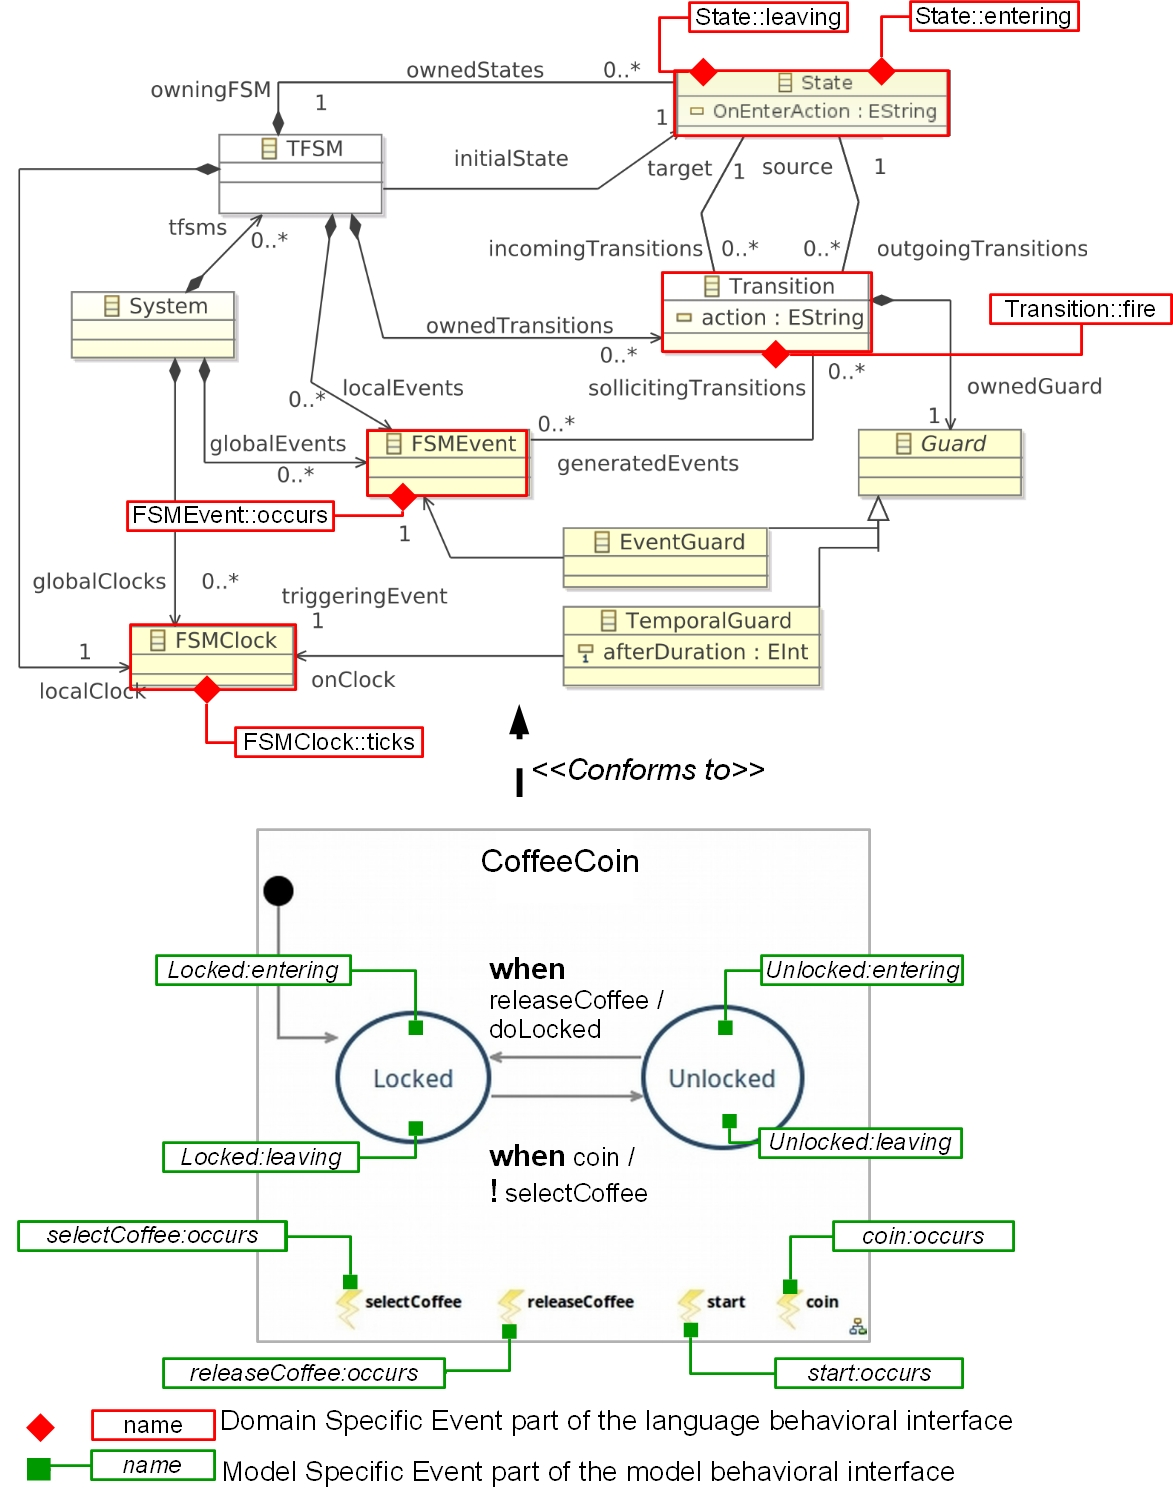
\includegraphics[width=1\textwidth]{bcool/figs/tfsmmm.jpg}
			\caption{(At the top) The TFSM metamodel with its language behavioral interface. (At the bottom) a TFSM model with its model behavioral interface}
			\label{fig:tfsmmm}
		\end{center}
	\end{figure}
	
	\begin{lstlisting}[language=ecl,
	caption={Partial \ecl specification of TFSM},
	label={fig:tfsmmmecl}, 
	basicstyle=\scriptsize\ttfamily, backgroundcolor=\color{LGrey}, numbers=left, xleftmargin=3pt]
	package tfsm
	context FSMClock
		def: ticks : Event = self
	context FSMEvent
		def: occurs : Event = self
	context State
		def : entering : Event = self
		def : leaving : Event = self
	\end{lstlisting}
	
The TFSM language defines the following \dse: \emph{entering} and \emph{leaving} a state, \emph{firing} a transition, the occurrences (\emph{occurs}) of a FSMEvent and the \emph{ticks} of a FSMClock (see at the top of Figure~\ref{fig:tfsmmm}). These \dse are part of the language behavioral interface of TFSM. % \dse are defined by using a specific language named \ecl (standing for Event Constraint Language~\cite{eclbib}) which is an extension of OCL~\cite{omgocl2bib} with events. \ecl takes benefits from the OCL query language and its possibility to augment an abstract syntax with additional attributes (without any side effects). Consequently, by using \ecl, it is possible to augment \as metaclasses and add \dse.
A partial \ecl specification of TFSM is shown in Listing~\ref{fig:tfsmmmecl} where the \dse \textit{entering} and \textit{leaving} are defined in the context of State (Listing~\ref{fig:tfsmmmecl}: line 6) while \textit{occurs} is defined in the context of FSMEvent (Listing~\ref{fig:tfsmmmecl}: line 4). When a metaclass is instantiated, the corresponding \dse are instantiated; \eg for each instance of the metaclass \emph{State}, \dse \textit{entering} is instantiated. Each instance of \dse is a \mse. 
	
We use the TFSM language to model the coin control system. We build a TFSM named \emph{CoffeeCoin} (At the button of Figure~\ref{fig:tfsmmm}). The model is composed of two states (\emph{Locked} and \emph{Unlocked}) and four FSMEvents (\emph{selectCoffee}, \emph{releaseCoffee}, \emph{start} and \emph{coin}). For each instance of state, a \dse \emph{entering} and \emph{leaving} are instantiated, \eg \emph{Locked:entering}, \emph{Locked:leaving}. Also, for each instance of FSMEvent, a \dse \emph{occurs} is instantiated, \eg \emph{releaseCoffee:occurs}, \emph{selectCoffee:occurs}. In the state Locked, when a coin is inserted (the \mse \emph{coin:occurs} happens), the TFSM becomes Unlocked and the \mse \emph{selectCoffee:occurs} is triggered. In state Unlocked, the release of the coffee (the \mse \emph{releaseCoffee:occurs} happens) makes the TFSM becomes Locked again.   
	
	\begin{figure}
		\begin{center}
			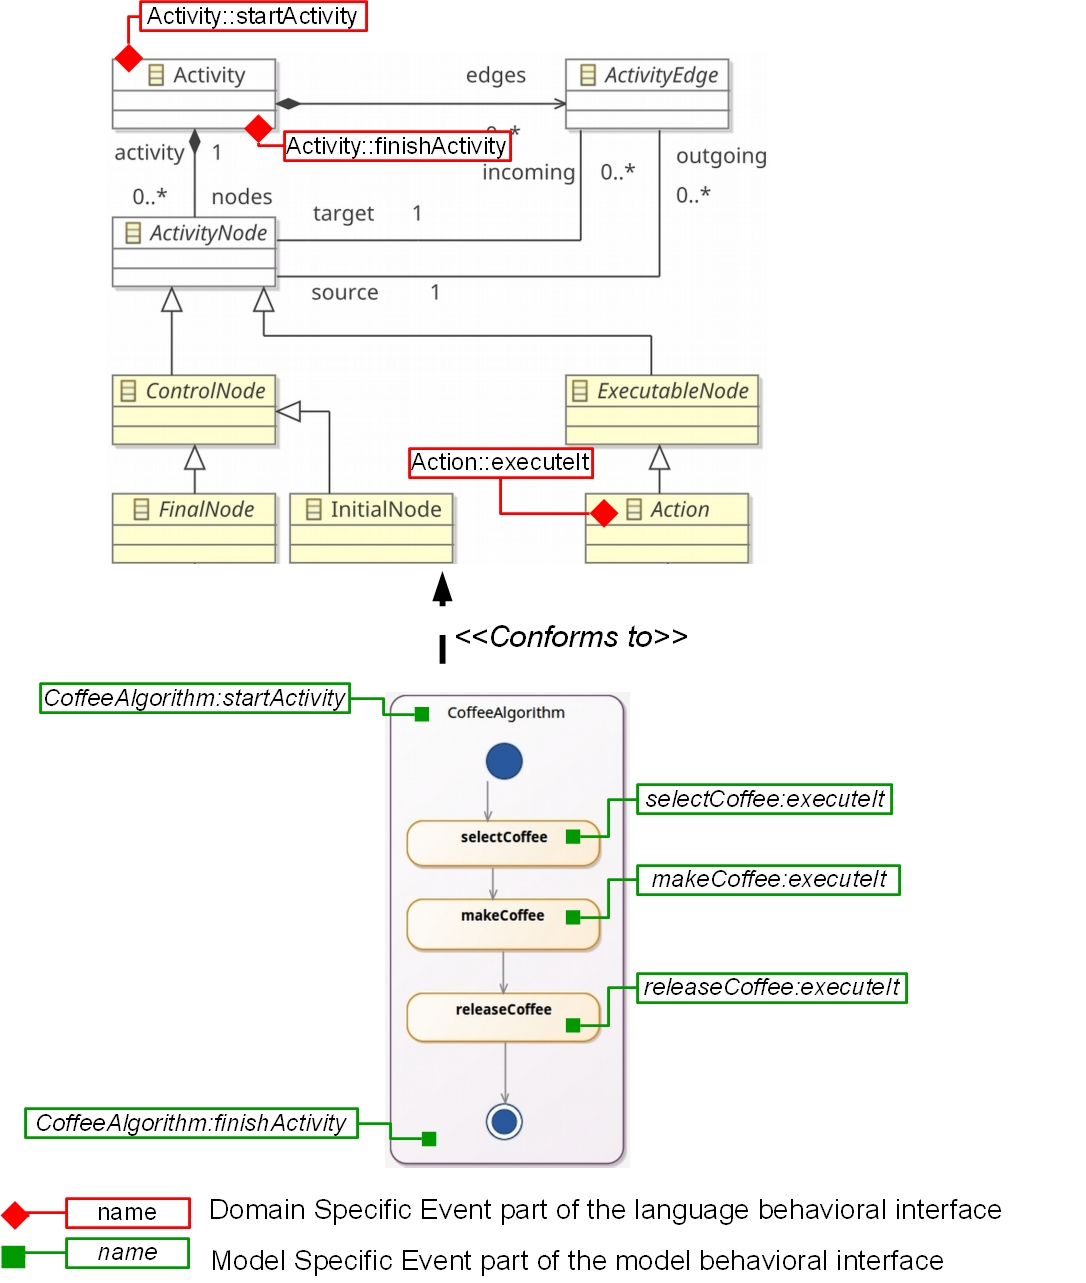
\includegraphics[width=1\textwidth]{bcool/figs/admm.jpg}
			\caption{(At the top) The Activity metamodel with its language behavioral interface. (At the bottom) an Activity model with its model behavioral interface}
			\label{fig:activitymm}
		\end{center}
	\end{figure}
	
	\begin{lstlisting}[language=ecl,
	caption={Partial \ecl specification of Activity Diagram},
	label={fig:eclfuml}, 
	basicstyle=\scriptsize\ttfamily, backgroundcolor=\color{LGrey}, numbers=left, xleftmargin=3pt, belowskip=-0.4em]
	package activitydiagram
	context Activity
		def: startActivity : Event = self
		def: finishActivity: Event = self
	context Action
		def : executeIt : Event = self
	\end{lstlisting}
To model the coffee algorithm system, we use the action-based language Activity~\cite{ttc15bib}. Figure~\ref{fig:activitymm} shows its partial metamodel. The root element is an \emph{Activity} that is composed of \emph{ActivityNodes} and \emph{ActivityEdges}. Each ActivityNode can be the source of outgoing ActivityEdges. The language behavioral interface of the Activity is partially shown in Listing~\ref{fig:eclfuml}. For each \emph{Activity} two \dse are defined: \emph{startActivity} and \emph{finishActivity}, to identify respectively the starting and finishing instants of the activity. One \dse is defined for each \emph{Action}: \emph{executeIt}, to identify the execution of an Action. At the button of Figure~\ref{fig:activitymm}, the activity named \emph{CoffeeAlgorithm} represents the simple algorithm for preparing coffee. It starts by the action \emph{selectCoffee} that asks the user to select the kind of coffee. After selected it (the \mse \emph{selectCoffee:executeIt} happens), the action \emph{makeCoffee} is executed. Finally, the coffee is released (the \mse \emph{releaseCoffee:executeIt} happens).

To represent the global behavior of the coffee machine, we have to specify how the TFSM \emph{CoffeeCoin} and the activity \emph{CoffeeAlgorithm} interact. More precisely, when the FSMEvent selectCoffee is triggered, the Action selectCoffee must be executed. Also, when the Action releaseCoffee is executed, the FSMEvent releaseCoffee must be triggered. To coordinate the execution of these models, we have to define some constraints between the \mse \emph{selectCoffee:occurs} and \emph{selectCoffee:executeIt}, and between \emph{releaseCoffee:occurs} and \emph{releaseCoffee:executeIt} (see Figure~\ref{fig:tfsmandadcoord}). We propose to generate these constraints by developing a simple \bcool operator between the TFSM and Activity language. We informally define the operator as follows: When coordinating a TFSM and an Activity, all pairs of FSMEvents and Actions that have the same name must be synchronized using a \emph{rendez-vous}. The operator is defined for any pair of TFSM and Activity, and specifies what and how instance of \dse \emph{occurs} and instances of \dse \emph{executeIt} must be coordinated. 

In this section, we have presented the TFSM and Activity languages that we used to build the heterogeneous model of a coffee machine. This resulted in two models: a TFSM named CoffeeCoin and an Activity named CoffeeAlgorithm. To get the global behavior of the coffee machine, we have proposed to specify some constraints between \mse of both models. Then, we have sketched a simple \bcool operator between the TFSM and Activity languages to generate such constrains. In the next section, we use this simple operator as running example to illustrate the syntax and semantics of \bcool. 

  
	\begin{figure}[h]
		\begin{center}
			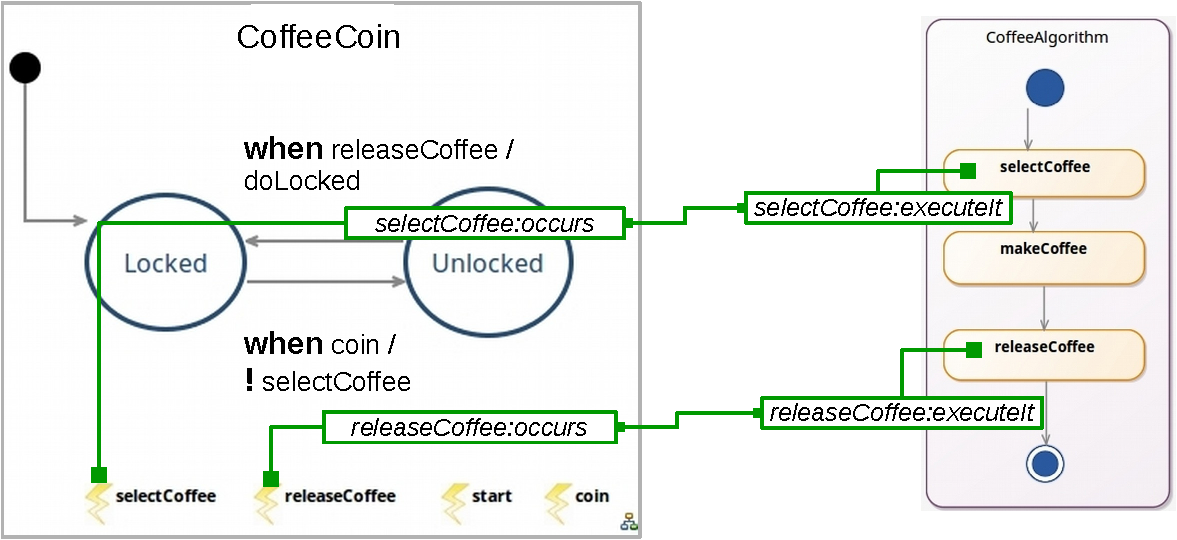
\includegraphics[width=1\textwidth]{bcool/figs/tfsmandadcoord}
			\caption{\mse of the models of the coffee machine to coordinate their execution}
			\label{fig:tfsmandadcoord}
		\end{center}
	\end{figure}

	%\item The model is composed by two States (\emph{Locked} and \emph{Unlocked}). So that there are two \mse of \textit{entering}: \textit{Locked} and \textit{Unlocked}. All \mse are part of the model behavioral interface. 